\documentclass[12pt,a4paper]{article}
\usepackage[utf8]{inputenc}
\usepackage[margin=1in]{geometry}
\usepackage{graphicx}
\usepackage{amsmath}
\usepackage{amsfonts}
\usepackage{amssymb}
\usepackage{xcolor}
\usepackage{listings}
\usepackage{tikz}
\usepackage{tcolorbox}
\usepackage{hyperref}
\usepackage{fontawesome5}
\usepackage{enumitem}
\usepackage{fancyhdr}
\usepackage{multicol}

% Custom colors
\definecolor{primaryblue}{RGB}{59, 130, 246}
\definecolor{secondarygreen}{RGB}{34, 197, 94}
\definecolor{accentorange}{RGB}{249, 115, 22}
\definecolor{lightgray}{RGB}{243, 244, 246}
\definecolor{darkgray}{RGB}{75, 85, 99}

% Custom boxes
\newtcolorbox{infobox}[1]{
    colback=lightgray,
    colframe=primaryblue,
    title=#1,
    fonttitle=\bfseries,
    rounded corners
}

\newtcolorbox{codebox}{
    colback=darkgray!10,
    colframe=darkgray,
    rounded corners,
    listing only,
    listing options={
        basicstyle=\ttfamily\small,
        breaklines=true
    }
}

% Custom commands
\newcommand{\feature}[2]{\textcolor{primaryblue}{\textbf{#1}}: #2}
\newcommand{\endpoint}[2]{\texttt{#1} & #2 \\}

% Header and footer
\pagestyle{fancy}
\fancyhf{}
\fancyhead[L]{\textcolor{primaryblue}{\textbf{Multi-Agent RAG Pipeline}}}
\fancyhead[R]{\thepage}
\fancyfoot[C]{\textcolor{darkgray}{\small FastAPI • LangChain • ChromaDB • Ollama • Next.js}}

\title{
    \vspace{-1cm}
    \Huge\textbf{\textcolor{primaryblue}{Multi-Agent FullStack RAG Pipeline}}\\
    \vspace{0.3cm}
    \Large\textcolor{darkgray}{Intelligent Agent Communication \& Real-time Evaluation System}\\
    \vspace{0.5cm}
    \large\textcolor{accentorange}{\textbf{LLM Assignment 3.1 \& 3.2}}
}

\author{
    \textbf{Anjila Subedi}\\
    \textcolor{darkgray}{Roll No: 29}\\
    \vspace{0.2cm}
    \textcolor{primaryblue}{Large Language Models Course}
}
\date{\today}

\begin{document}

\maketitle

\begin{abstract}
A comprehensive multi-agent RAG system featuring intelligent agent communication, real-time evaluation metrics, and advanced content processing capabilities. The system implements a message bus architecture with specialized agents for document processing, web scraping, and quality evaluation.

\textbf{Assignment Context:} This project demonstrates advanced implementation of Large Language Model concepts including multi-agent systems, retrieval-augmented generation (RAG), real-time evaluation metrics, and intelligent agent communication patterns as part of LLM Assignment 3.1 and 3.2.
\end{abstract}

\section{Assignment Overview}

\begin{infobox}{LLM Assignment 3.1 \& 3.2 - Multi-Agent RAG System}
\textbf{Student:} Anjila Subedi (Roll No: 29)\\
\textbf{Course:} Large Language Models\\
\textbf{Assignment Focus:} Implementation of advanced RAG systems with multi-agent architecture

\textbf{Key Learning Objectives Demonstrated:}
\begin{itemize}
    \item Multi-agent system design and implementation
    \item Real-time evaluation metrics for LLM outputs
    \item Advanced retrieval-augmented generation techniques
    \item Agent communication and coordination patterns
    \item Performance monitoring and quality assessment
\end{itemize}
\end{infobox}

\subsection{Assignment 3.1: Multi-Agent Architecture Design}

This assignment focuses on designing and implementing a sophisticated multi-agent system that demonstrates:

\begin{enumerate}
    \item \textbf{Agent Specialization}: Each agent has a specific role (Document Processing, Web Scraping, Evaluation, System Coordination)
    \item \textbf{Communication Patterns}: Implementation of message bus architecture for inter-agent communication
    \item \textbf{Shared Memory Systems}: Centralized data sharing between agents
    \item \textbf{Asynchronous Processing}: Non-blocking agent operations and parallel processing capabilities
\end{enumerate}

\subsection{Assignment 3.2: RAG Evaluation Framework}

This assignment demonstrates advanced evaluation techniques for RAG systems:

\begin{enumerate}
    \item \textbf{Multi-Metric Assessment}: Implementation of 4 key evaluation metrics
    \item \textbf{Real-time Evaluation}: Instant quality feedback for LLM responses
    \item \textbf{Automated Quality Control}: Systematic assessment of answer quality
    \item \textbf{Performance Analytics}: Comprehensive evaluation reporting and insights
\end{enumerate}

\section{Key Features}

\begin{itemize}[leftmargin=0.5cm]
    \item \feature{Multi-Agent Communication}{Message bus architecture with shared memory}
    \item \feature{Real-time Evaluation}{4-metric assessment system with detailed feedback}
    \item \feature{Advanced Content Processing}{PDF and web content extraction}
    \item \feature{Performance Monitoring}{Agent activity tracking and health monitoring}
    \item \feature{Modern UI}{Next.js frontend with evaluation interface}
\end{itemize}

\section{System Workflow}

\subsection{Step 1: Content Upload \& Processing}

\begin{figure}[h]
    \centering
    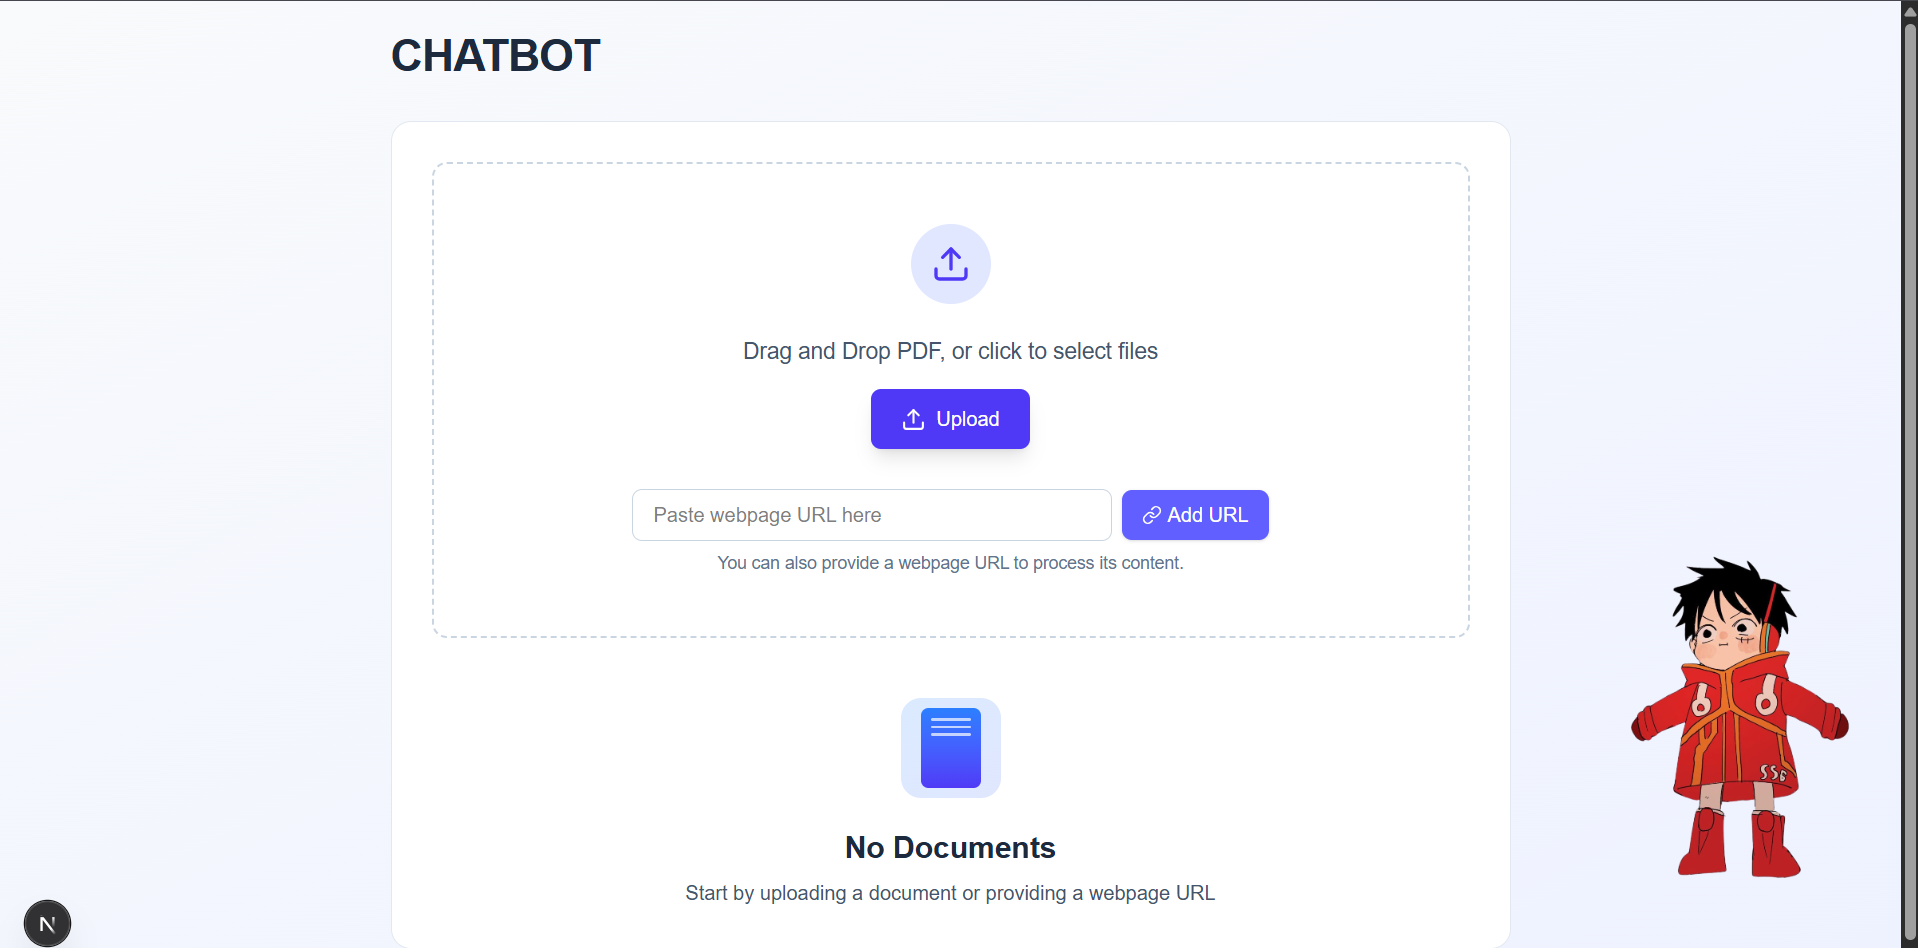
\includegraphics[width=0.8\textwidth]{screenshots/landing_page.png}
    \caption{Content Upload Interface}
\end{figure}

\begin{infobox}{Process Flow}
\centering
\texttt{User Upload → Document Agent → Text Chunking → Vector Storage → Ready for Queries}
\end{infobox}

\subsection{Step 2: Interactive Chat Interface}

\begin{figure}[h]
    \centering
    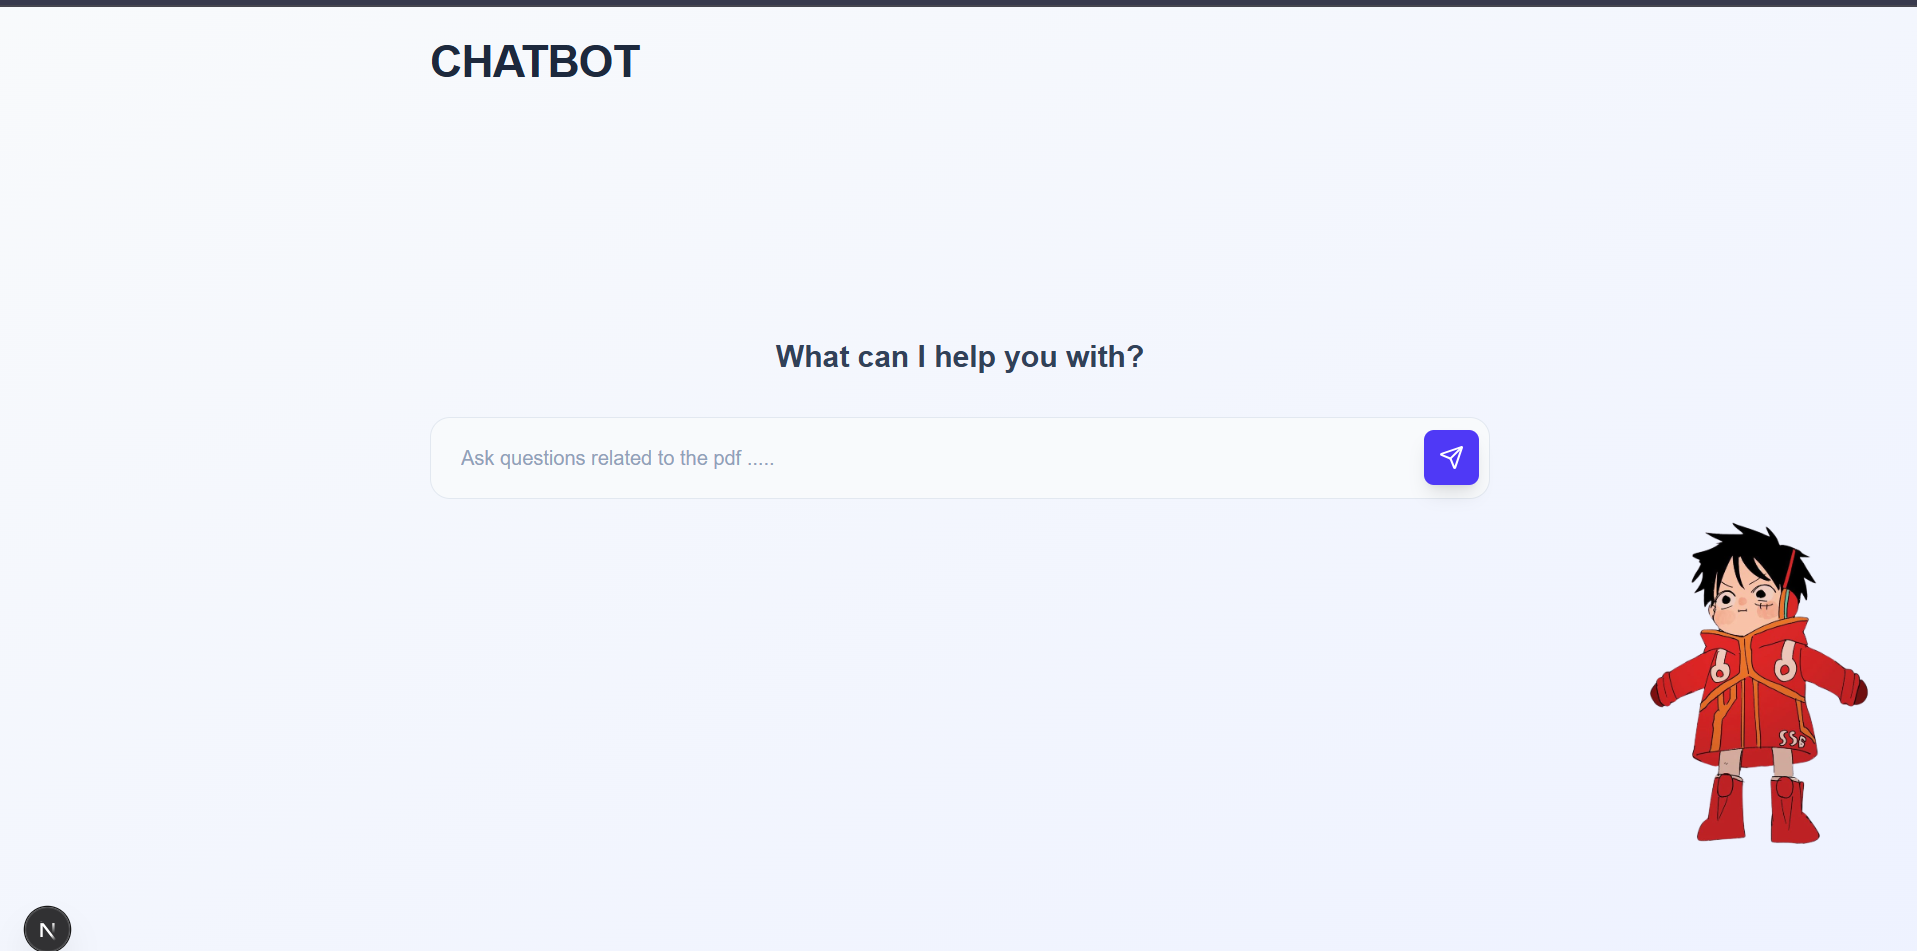
\includegraphics[width=0.8\textwidth]{screenshots/chat_page.png}
    \caption{Interactive Chat Interface}
\end{figure}

\textbf{Chat Features:}
\begin{itemize}
    \item Real-time messaging with markdown support
    \item Evaluation toggle for quality assessment
    \item Ground truth input for correctness testing
\end{itemize}

\subsection{Step 3: Intelligent Query Processing}

\begin{figure}[h]
    \centering
    \begin{minipage}{0.45\textwidth}
        \centering
        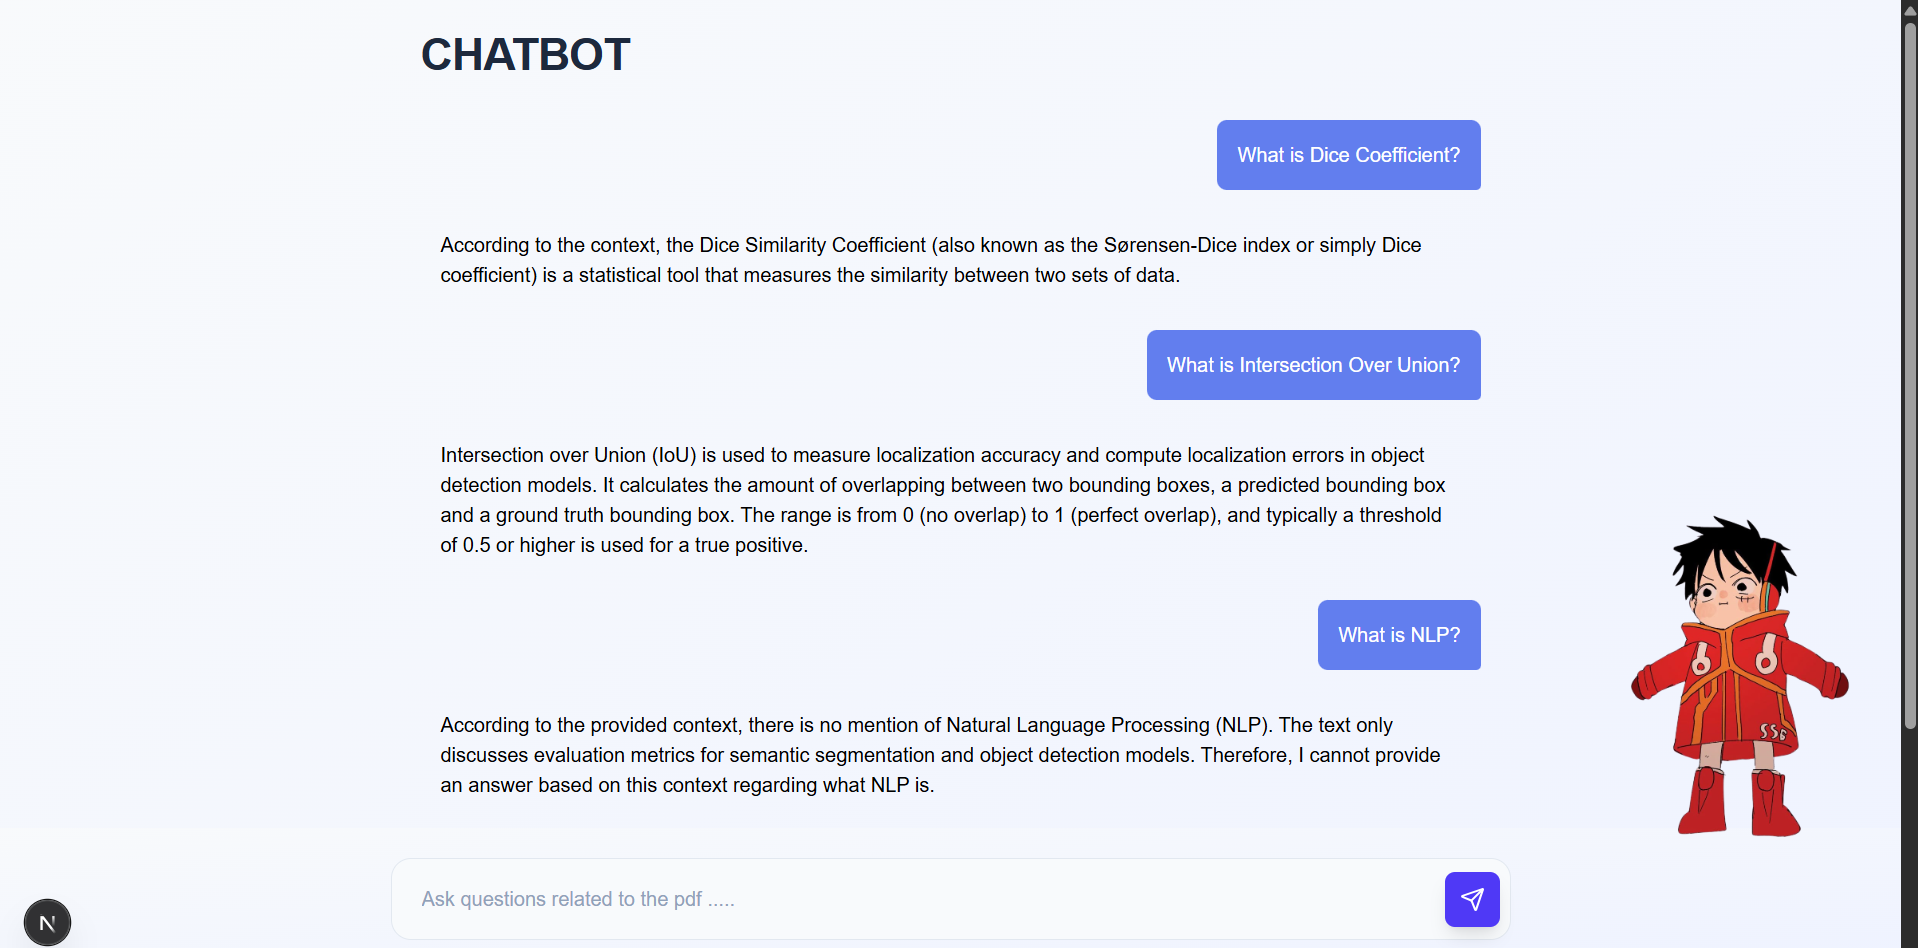
\includegraphics[width=\textwidth]{screenshots/pdf_answers.png}
        \caption{PDF Processing Example}
    \end{minipage}
    \hfill
    \begin{minipage}{0.45\textwidth}
        \centering
        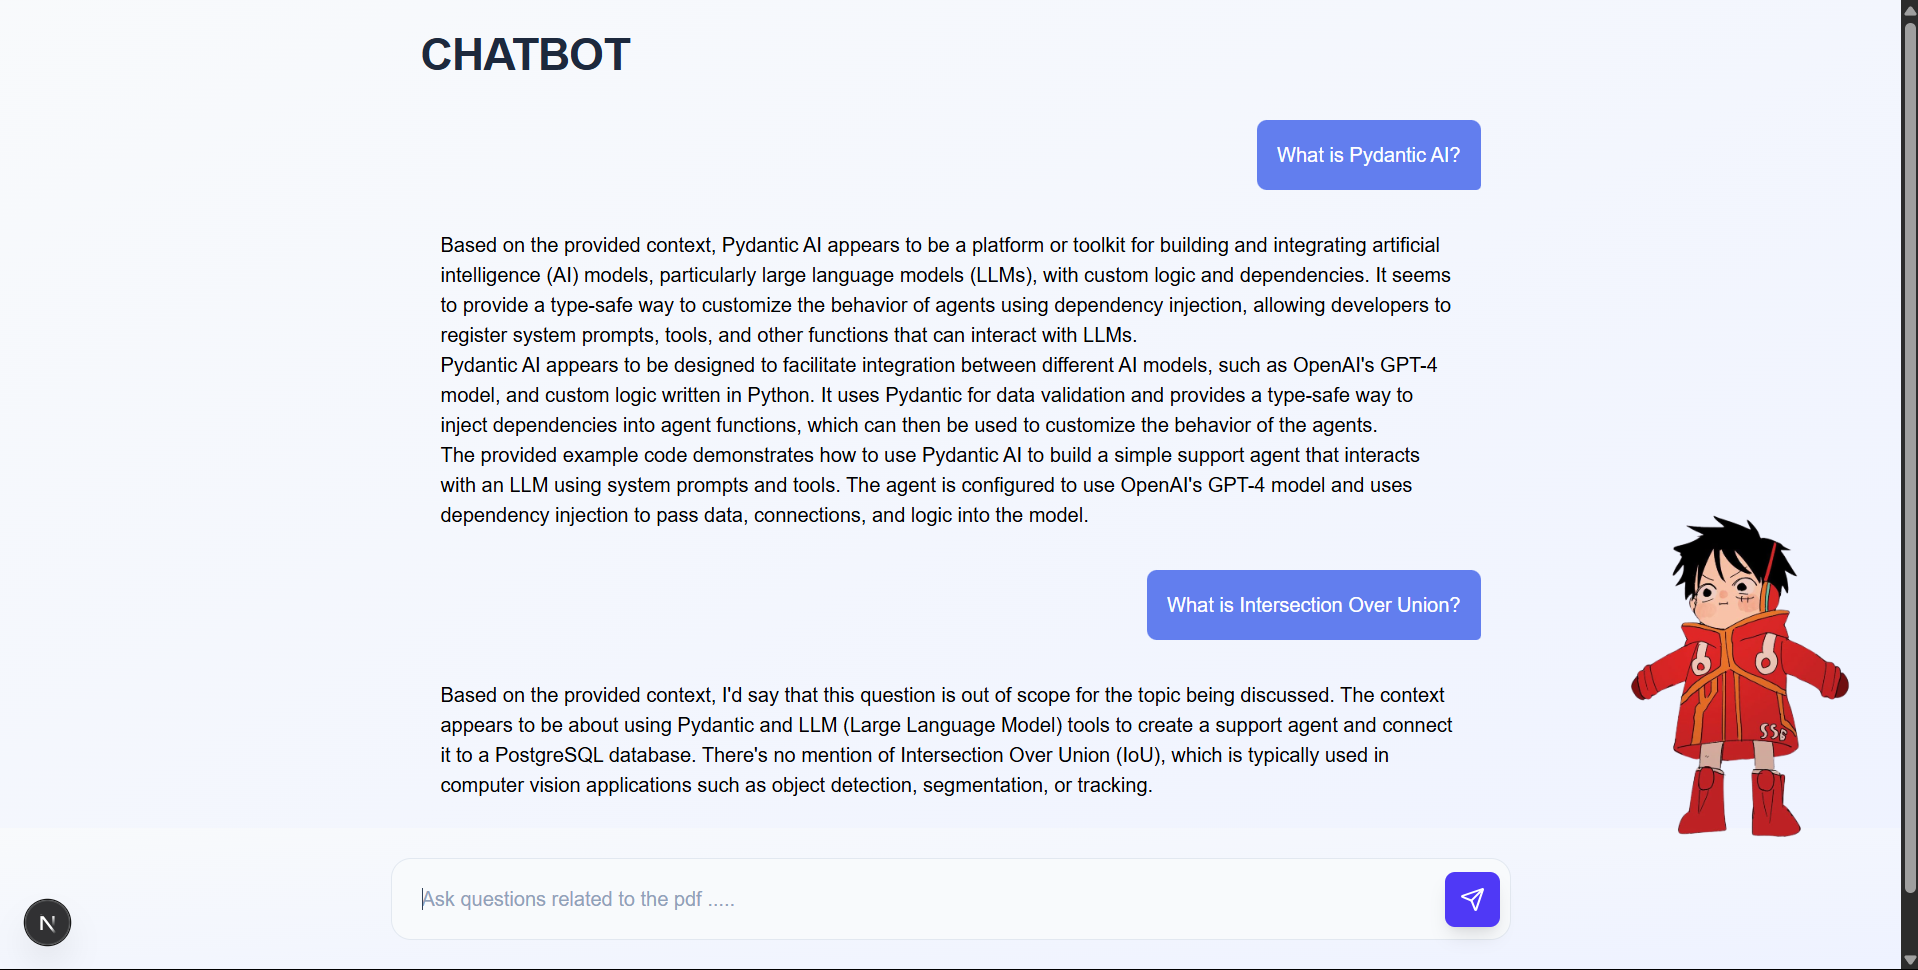
\includegraphics[width=\textwidth]{screenshots/url_answers.png}
        \caption{Web Content Processing}
    \end{minipage}
\end{figure}

\subsection{Step 4: Real-time Evaluation System}

\begin{figure}[h]
    \centering
    \begin{minipage}{0.45\textwidth}
        \centering
        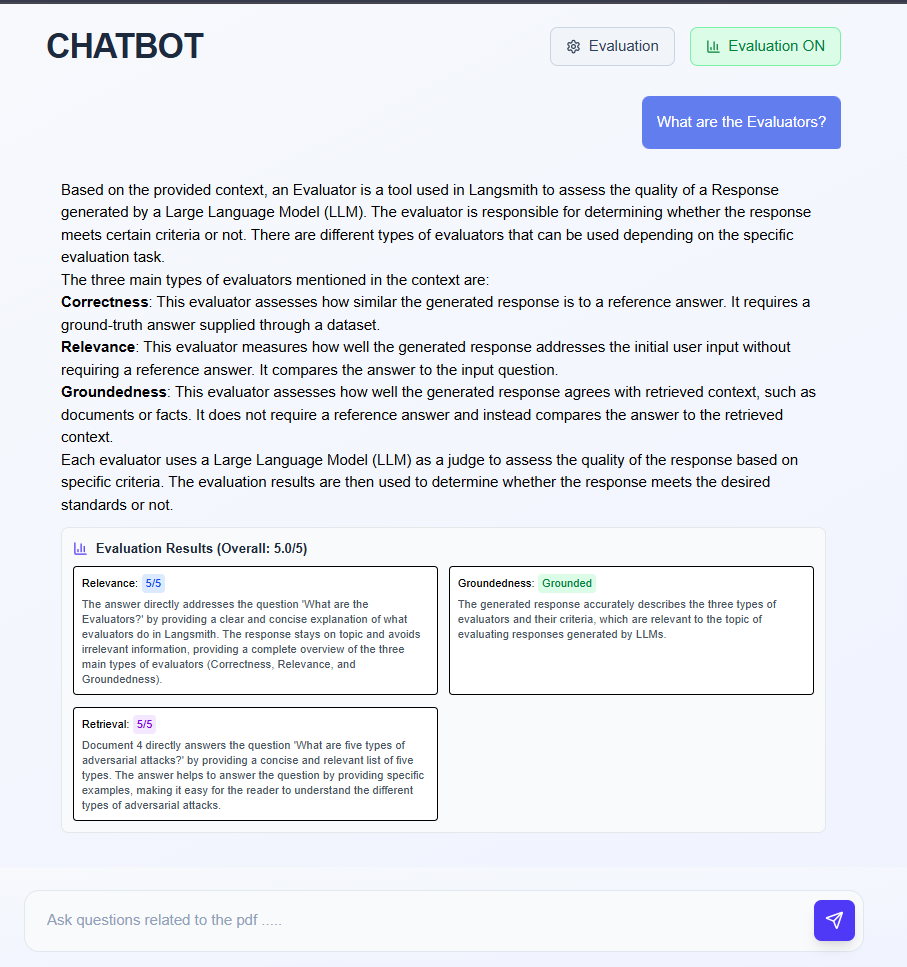
\includegraphics[width=\textwidth]{screenshots/eval.png}
        \caption{Evaluation Interface}
    \end{minipage}
    \hfill
    \begin{minipage}{0.45\textwidth}
        \centering
        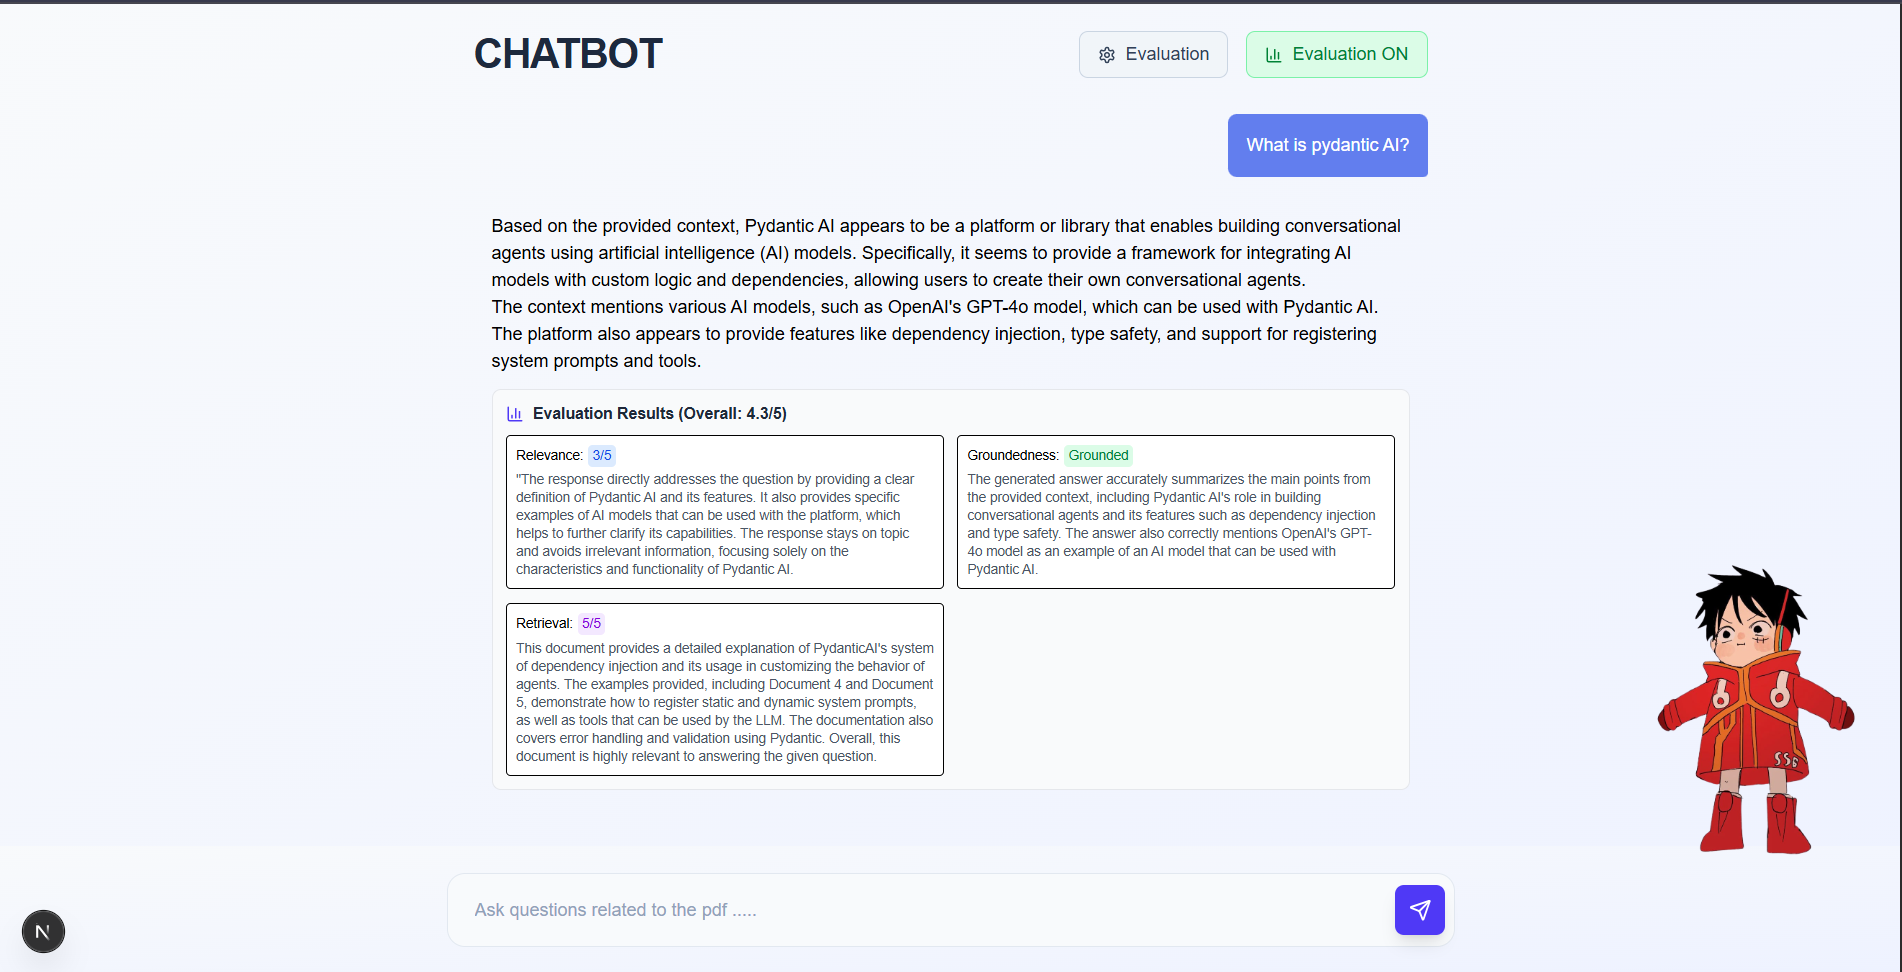
\includegraphics[width=\textwidth]{screenshots/evaluation.png}
        \caption{Detailed Evaluation Results}
    \end{minipage}
\end{figure}

\textbf{Evaluation Metrics:}
\begin{itemize}
    \item \textcolor{secondarygreen}{\textbf{Correctness}}: Answer accuracy against ground truth
    \item \textcolor{primaryblue}{\textbf{Relevance}}: Question-answer alignment (1-5 scale)
    \item \textcolor{accentorange}{\textbf{Groundedness}}: Context-based answer validation
    \item \textcolor{darkgray}{\textbf{Retrieval Quality}}: Document relevance assessment
\end{itemize}

\newpage

\section{Multi-Agent Architecture}

\subsection{System Architecture Overview}

\begin{figure}[h]
\centering
\begin{tikzpicture}[
    agent/.style={draw, rectangle, minimum width=2.5cm, minimum height=1.5cm, rounded corners, fill=lightgray},
    coordinator/.style={draw, rectangle, minimum width=2.5cm, minimum height=1cm, rounded corners, fill=primaryblue!20},
    memory/.style={draw, rectangle, minimum width=2.5cm, minimum height=1cm, rounded corners, fill=secondarygreen!20},
    orchestrator/.style={draw, rectangle, minimum width=2.5cm, minimum height=1.5cm, rounded corners, fill=accentorange!20},
    arrow/.style={->, thick, color=darkgray}
]

% Agents
\node[agent] (doc) at (0,4) {Document Agent};
\node[agent] (web) at (4,4) {Web Scraping Agent};
\node[agent] (eval) at (8,4) {Evaluation Agent};

% Central components
\node[coordinator] (bus) at (2,2) {Message Bus Coordinator};
\node[memory] (memory) at (6,2) {Shared Memory Store};

% Main orchestrator
\node[orchestrator] (orch) at (4,0) {RAG Orchestrator (Main API)};

% Connections
\draw[arrow] (doc) -- (bus);
\draw[arrow] (web) -- (bus);
\draw[arrow] (eval) -- (bus);
\draw[arrow] (doc) -- (memory);
\draw[arrow] (web) -- (memory);
\draw[arrow] (eval) -- (memory);
\draw[arrow] (bus) -- (orch);

\end{tikzpicture}
\caption{Multi-Agent System Architecture}
\end{figure}

\subsection{Agent Communication Flow}

\begin{infobox}{Message Bus System}
\begin{itemize}
    \item \textbf{Centralized Hub}: All agents communicate through a single message bus
    \item \textbf{Async Messaging}: Non-blocking message passing between agents
    \item \textbf{Event Broadcasting}: Status updates propagated to all interested agents
\end{itemize}
\end{infobox}

\begin{codebox}
\begin{lstlisting}[language=Python, caption=Shared Memory Architecture]
# Agent A stores data
shared_memory.set("pdf_chunks", processed_data)

# Agent B retrieves data
data = shared_memory.get("pdf_chunks")
\end{lstlisting}
\end{codebox}

\textbf{Agent Coordination Example:}
\begin{enumerate}
    \item Document Agent: "PDF processing started"
    \item Message Bus: Broadcast to System Coordinator
    \item Shared Memory: Store processing results
    \item Evaluation Agent: "Ready for evaluation"
    \item System Coordinator: "Pipeline ready"
\end{enumerate}

\subsection{Specialized Agent Roles}

\begin{multicols}{2}
\textbf{Document Processing Agent}
\begin{itemize}
    \item PDF text extraction and chunking
    \item Metadata preservation
    \item Status reporting to message bus
\end{itemize}

\textbf{Web Scraping Agent}
\begin{itemize}
    \item Async HTTP requests
    \item HTML parsing and cleaning
    \item Content validation and storage
\end{itemize}

\textbf{Evaluation Agent}
\begin{itemize}
    \item Multi-metric assessment
    \item Real-time quality scoring
    \item Detailed feedback generation
\end{itemize}

\textbf{System Coordinator}
\begin{itemize}
    \item Agent health monitoring
    \item Activity logging
    \item Error handling and recovery
\end{itemize}
\end{multicols}

\newpage

\section{Evaluation Process Deep Dive}

\subsection{4-Metric Assessment System}

\begin{figure}[h]
\centering
\begin{tikzpicture}[
    metric/.style={draw, rectangle, minimum width=2cm, minimum height=1cm, rounded corners, fill=lightgray},
    process/.style={draw, ellipse, minimum width=1.5cm, minimum height=0.8cm, fill=primaryblue!20},
    arrow/.style={->, thick}
]

% Metrics
\node[metric] (correct) at (0,6) {Correctness};
\node[metric] (relevance) at (3,6) {Relevance};
\node[metric] (ground) at (6,6) {Groundedness};
\node[metric] (retrieval) at (9,6) {Retrieval};

% Processing
\node[process] (llm) at (0,4) {LLM Analysis};
\node[process] (score) at (3,4) {Score 1-5};
\node[process] (context) at (6,4) {Context Check};
\node[process] (doc) at (9,4) {Document Score};

% Results
\node[metric, fill=secondarygreen!20] (binary1) at (0,2) {Binary};
\node[metric, fill=primaryblue!20] (numerical1) at (3,2) {Numerical};
\node[metric, fill=accentorange!20] (binary2) at (6,2) {Binary};
\node[metric, fill=darkgray!20] (numerical2) at (9,2) {Numerical};

% Combined result
\node[metric, fill=accentorange!30] (combined) at (4.5,0) {Combined Overall Score};

% Arrows
\draw[arrow] (correct) -- (llm);
\draw[arrow] (relevance) -- (score);
\draw[arrow] (ground) -- (context);
\draw[arrow] (retrieval) -- (doc);

\draw[arrow] (llm) -- (binary1);
\draw[arrow] (score) -- (numerical1);
\draw[arrow] (context) -- (binary2);
\draw[arrow] (doc) -- (numerical2);

\draw[arrow] (binary1) -- (combined);
\draw[arrow] (numerical1) -- (combined);
\draw[arrow] (binary2) -- (combined);
\draw[arrow] (numerical2) -- (combined);

\end{tikzpicture}
\caption{Evaluation Workflow Architecture}
\end{figure}

\subsection{Evaluation Metrics Details}

\begin{infobox}{Correctness Evaluation}
\texttt{Ground Truth Input → LLM Comparison → Binary Score (✓/✗)}
\begin{itemize}
    \item Semantic similarity analysis
    \item Factual accuracy check
    \item Key information coverage
\end{itemize}
\end{infobox}

\begin{infobox}{Relevance Scoring (1-5 Scale)}
\texttt{Question Analysis → Answer Relevance → Numerical Score}
\begin{itemize}
    \item Topic alignment verification
    \item Context appropriateness
    \item Response completeness
\end{itemize}
\end{infobox}

\begin{infobox}{Groundedness Assessment}
\texttt{Retrieved Context → Answer Validation → Support Score}
\begin{itemize}
    \item Citation accuracy check
    \item Hallucination detection
    \item Source material alignment
\end{itemize}
\end{infobox}

\begin{infobox}{Retrieval Quality (1-5 Scale)}
\texttt{Query Vector → Document Matching → Relevance Score}
\begin{itemize}
    \item Semantic similarity measurement
    \item Content coverage analysis
    \item Information completeness
\end{itemize}
\end{infobox}

\section{API Endpoints}

\subsection{Core Operations}
\begin{tabular}{|l|l|}
\hline
\textbf{Endpoint} & \textbf{Description} \\
\hline
\endpoint{POST /upload}{PDF processing via Document Agent}
\endpoint{POST /url}{Web content via Scraping Agent}
\endpoint{POST /query}{Standard RAG queries}
\endpoint{POST /query\_with\_evaluation}{Queries with real-time evaluation}
\endpoint{DELETE /clear}{Clear vector database}
\hline
\end{tabular}

\subsection{Evaluation Endpoints}
\begin{tabular}{|l|l|}
\hline
\textbf{Endpoint} & \textbf{Description} \\
\hline
\endpoint{POST /evaluate/correctness}{Binary accuracy assessment}
\endpoint{POST /evaluate/relevance}{1-5 scale relevance scoring}
\endpoint{POST /evaluate/groundedness}{Context support validation}
\endpoint{POST /evaluate/complete}{Full 4-metric evaluation}
\endpoint{GET /evaluator/health}{Evaluation system status}
\hline
\end{tabular}

\subsection{Agent Monitoring}
\begin{tabular}{|l|l|}
\hline
\textbf{Endpoint} & \textbf{Description} \\
\hline
\endpoint{GET /agents/status}{Real-time agent health}
\endpoint{GET /agents/activities}{Recent agent activity logs}
\endpoint{GET /agents/shared\_data}{Shared memory inspection}
\hline
\end{tabular}

\section{Quick Start}

\subsection{Backend Setup}
\begin{codebox}
\begin{lstlisting}[language=bash]
# Install dependencies
pip install -r backend/requirements.txt

# Start FastAPI server
cd backend && python rag.py

# Verify Ollama models
ollama list | grep -E "(mxbai-embed-large|llama3)"
\end{lstlisting}
\end{codebox}

\subsection{Frontend Setup}
\begin{codebox}
\begin{lstlisting}[language=bash]
# Install and start Next.js
cd chatbot
npm install && npm run dev
\end{lstlisting}
\end{codebox}

\subsection{Access Points}
\begin{itemize}
    \item \textbf{Frontend}: \url{http://localhost:3000}
    \item \textbf{API Docs}: \url{http://localhost:8000/docs}
    \item \textbf{Agent Status}: \url{http://localhost:8000/agents/status}
\end{itemize}

\section{System Benefits}

\begin{multicols}{2}
\begin{itemize}
    \item[\textcolor{secondarygreen}{\checkmark}] \textbf{Modular Architecture}: Independent, specialized agents
    \item[\textcolor{secondarygreen}{\checkmark}] \textbf{Real-time Evaluation}: Instant quality feedback
    \item[\textcolor{secondarygreen}{\checkmark}] \textbf{Transparent Operations}: Complete activity visibility
    \item[\textcolor{secondarygreen}{\checkmark}] \textbf{Scalable Design}: Easy agent addition and modification
    \item[\textcolor{secondarygreen}{\checkmark}] \textbf{Robust Error Handling}: Isolated failure management
    \item[\textcolor{secondarygreen}{\checkmark}] \textbf{Modern UI/UX}: Responsive design with rich interactions
\end{itemize}
\end{multicols}

\section{Assignment Reflection \& Learning Outcomes}

\subsection{Technical Achievements}

\begin{infobox}{Assignment 3.1 Accomplishments}
\textbf{Multi-Agent System Implementation:}
\begin{itemize}
    \item Successfully designed and implemented 4 specialized agents
    \item Created robust message bus communication system
    \item Implemented shared memory architecture for data persistence
    \item Achieved asynchronous processing with proper error handling
\end{itemize}
\end{infobox}

\begin{infobox}{Assignment 3.2 Accomplishments}
\textbf{RAG Evaluation Framework:}
\begin{itemize}
    \item Developed comprehensive 4-metric evaluation system
    \item Implemented real-time quality assessment capabilities
    \item Created detailed feedback mechanisms with explanations
    \item Built performance tracking and analytics dashboard
\end{itemize}
\end{infobox}

\subsection{Key Learning Insights}

\textbf{1. Multi-Agent Coordination Complexity}
\begin{itemize}
    \item Understanding the challenges of distributed system design
    \item Learning effective inter-agent communication patterns
    \item Managing state consistency across multiple agents
\end{itemize}

\textbf{2. RAG System Evaluation Challenges}
\begin{itemize}
    \item Implementing objective quality metrics for subjective responses
    \item Balancing automated evaluation with human judgment
    \item Creating meaningful performance benchmarks
\end{itemize}

\textbf{3. System Integration \& Scalability}
\begin{itemize}
    \item Building modular systems that can grow and adapt
    \item Implementing proper error isolation and recovery
    \item Creating maintainable and extensible architectures
\end{itemize}

\subsection{Future Enhancements}

\textbf{Potential Improvements for Advanced LLM Applications:}
\begin{enumerate}
    \item \textbf{Advanced Agent Reasoning}: Implement chain-of-thought processing
    \item \textbf{Dynamic Agent Spawning}: Create agents on-demand based on workload
    \item \textbf{Multi-Modal Processing}: Extend to handle images, audio, and video
    \item \textbf{Federated Learning}: Implement distributed model training capabilities
    \item \textbf{Advanced Evaluation Metrics}: Include bias detection and fairness assessment
\end{enumerate}

\vspace{1cm}
\begin{center}
\textbf{\large Technology Stack}\\
\vspace{0.3cm}
\textcolor{primaryblue}{FastAPI} • \textcolor{secondarygreen}{LangChain} • \textcolor{accentorange}{ChromaDB} • \textcolor{darkgray}{Ollama} • \textcolor{primaryblue}{Next.js} • \textcolor{secondarygreen}{TypeScript}
\end{center}

\vspace{0.5cm}
\begin{center}
\textcolor{darkgray}{\small Submitted by: \textbf{Anjila Subedi} | Roll No: 29 | LLM Assignment 3.1 \& 3.2}
\end{center>

\end{document}
